\documentclass{article}
\usepackage{amsmath}
\usepackage{amssymb}
\usepackage{graphicx}
\author{Cláudio Ferreira Carneiro - RA 263796}
\title{EFC 1}
\begin{document}
    \maketitle
    \pagenumbering{gobble}
    \newpage
    \pagenumbering{arabic}
    \section[]{Atividades teóricas}
    \section[]{Atividades computacionais}
    Nesta atividade é utilizado o \textit{dataset} contendo a temperatura mínima
    diária em Melbourne, Austrália, no período de 1981 a 1990 \ref{fig:dataset}. As amostras do ano
    de 1990 foram reservadas para testes e o restante para treinamento e validação:
    \begin{figure}[!h]
        \centering
        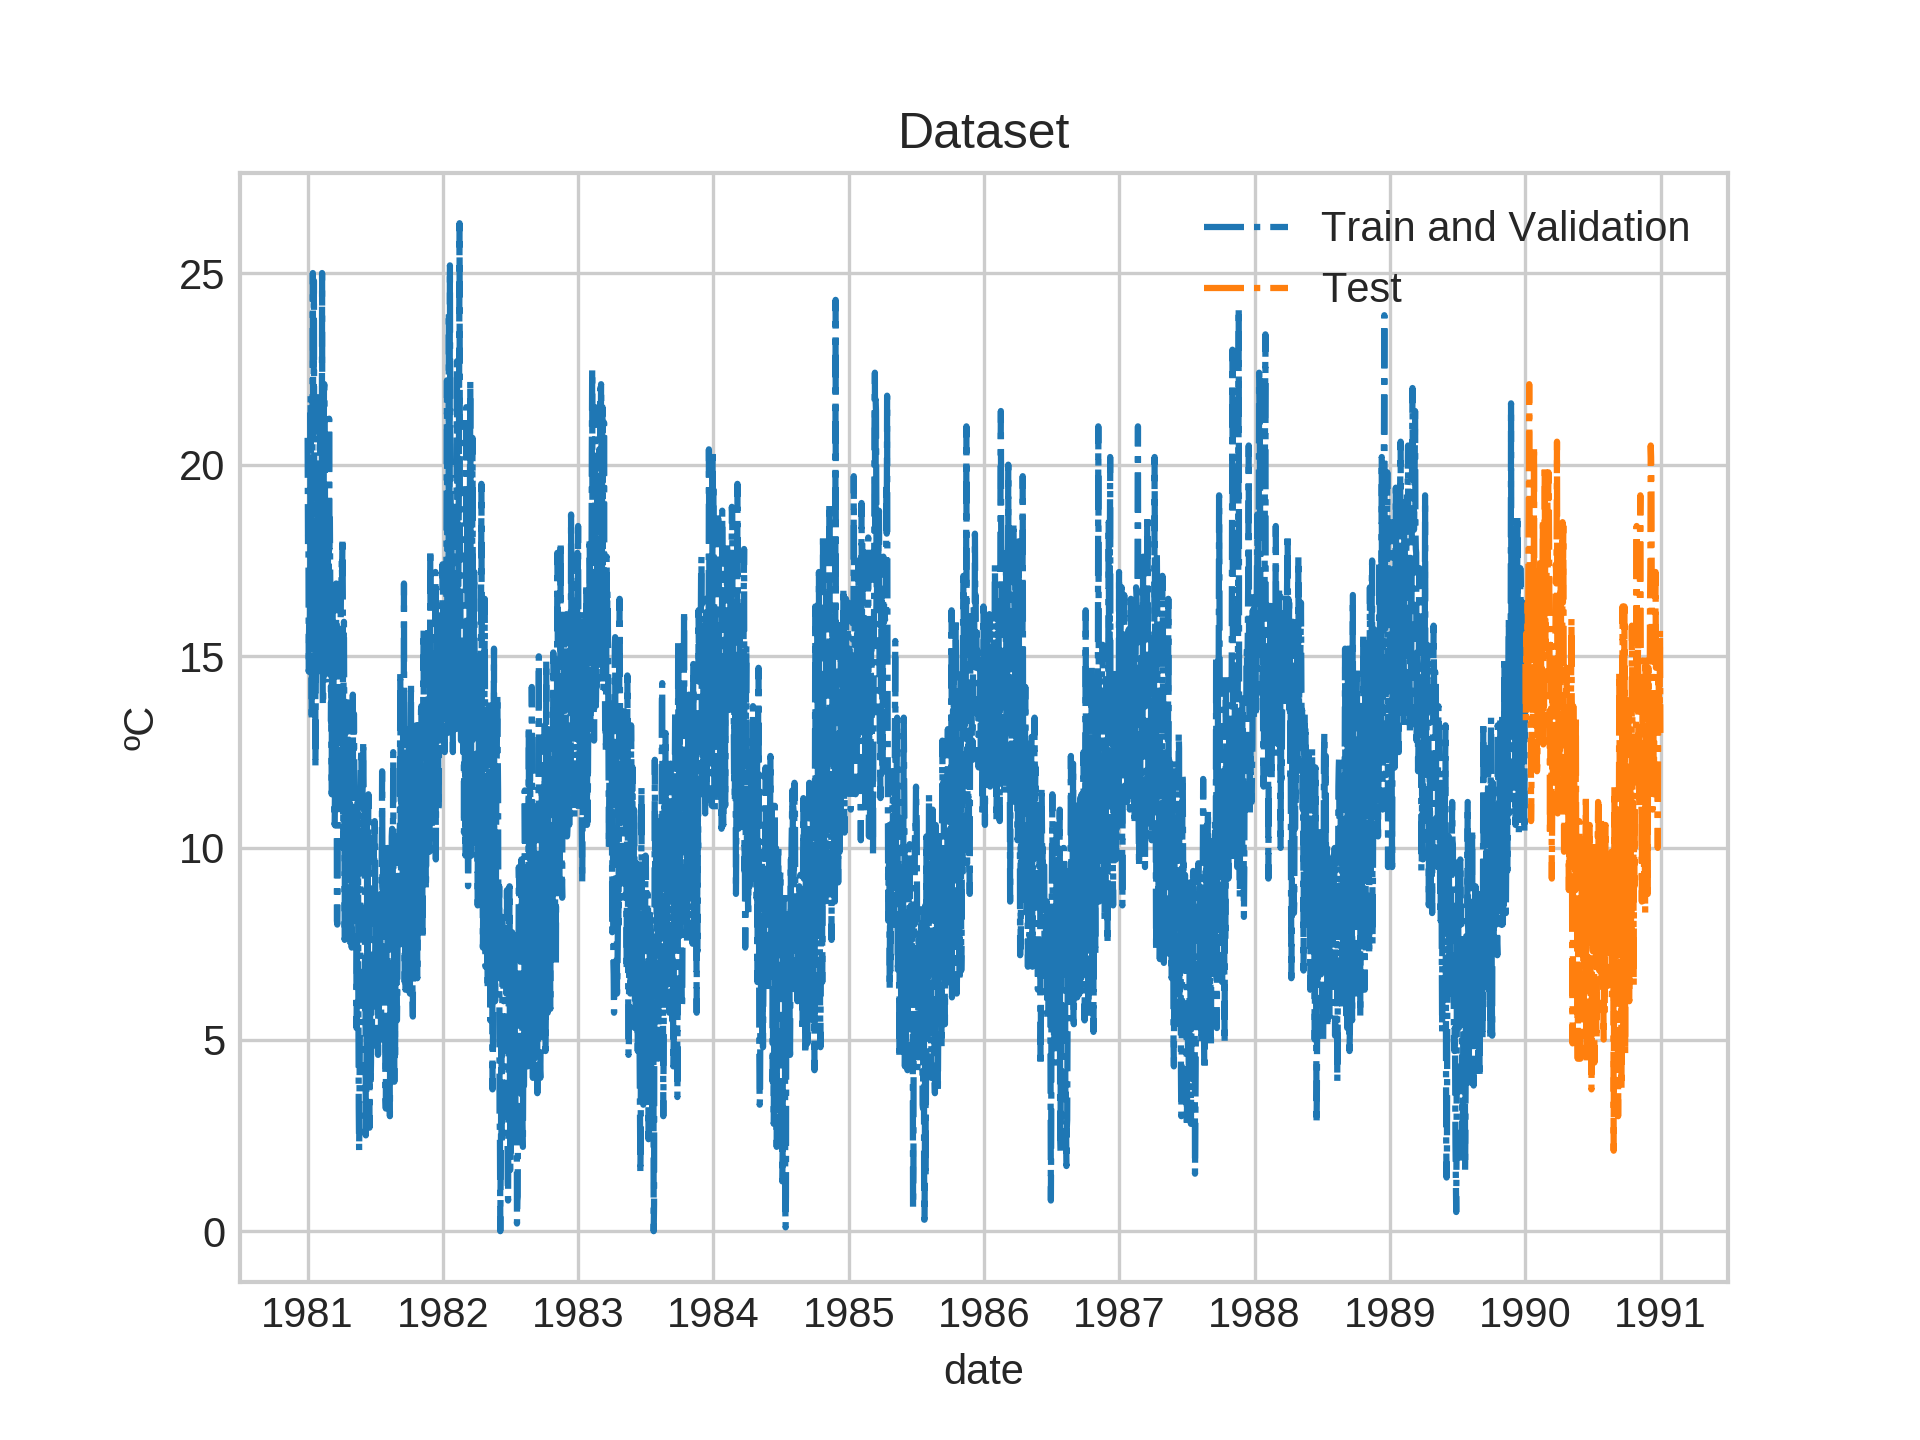
\includegraphics[width=\linewidth]{ex01/dataset.png}
        \caption{Temperatura mínima diária em Melbourne, Austrália, no período de 1981 a 1990.}
        \label{fig:dataset}
    \end{figure}
    \subsection[]{Exercício 01}
    A obtenção do valor ótimo da quantidade de atrasos da série temporal ($K$), 
    é condicionado ao resultado da validação do modelo em questão. Portanto, torna-se 
    necessário que esta validação esteja isenta de vícios e apresente uma visão tão próxima
    quanto possível da dinâmica do modelo. Para isso é aplicada a técnica de validação cruzada
    \textit{k-fold}, sendo $k$ o número de partes, $folds$.

    O número de \textit{folds} utilizado na validação do modelo foi definido como $k=10$ por ser um valor
    típico e separar para validação \textit{datasets} de comprimento próximo ao número de dias no ano,
    possibilitando que a dinâmica anual da temperatura esteja representada. 
    
    Nota-se que a quantidade de atrasos (atributos) influencia o desempenho do modelo de forma considerável
    porém não possui uma relação linear com o RMSE da estimação \ref{fig:ex1_kfold_rmse}. Ganhos consideráveis são obtidos até certo
    valor de $K$ e logo após o RMSE, de forma menos abrupta, torna a aumentar.
    \begin{figure}[!h]
        \centering
        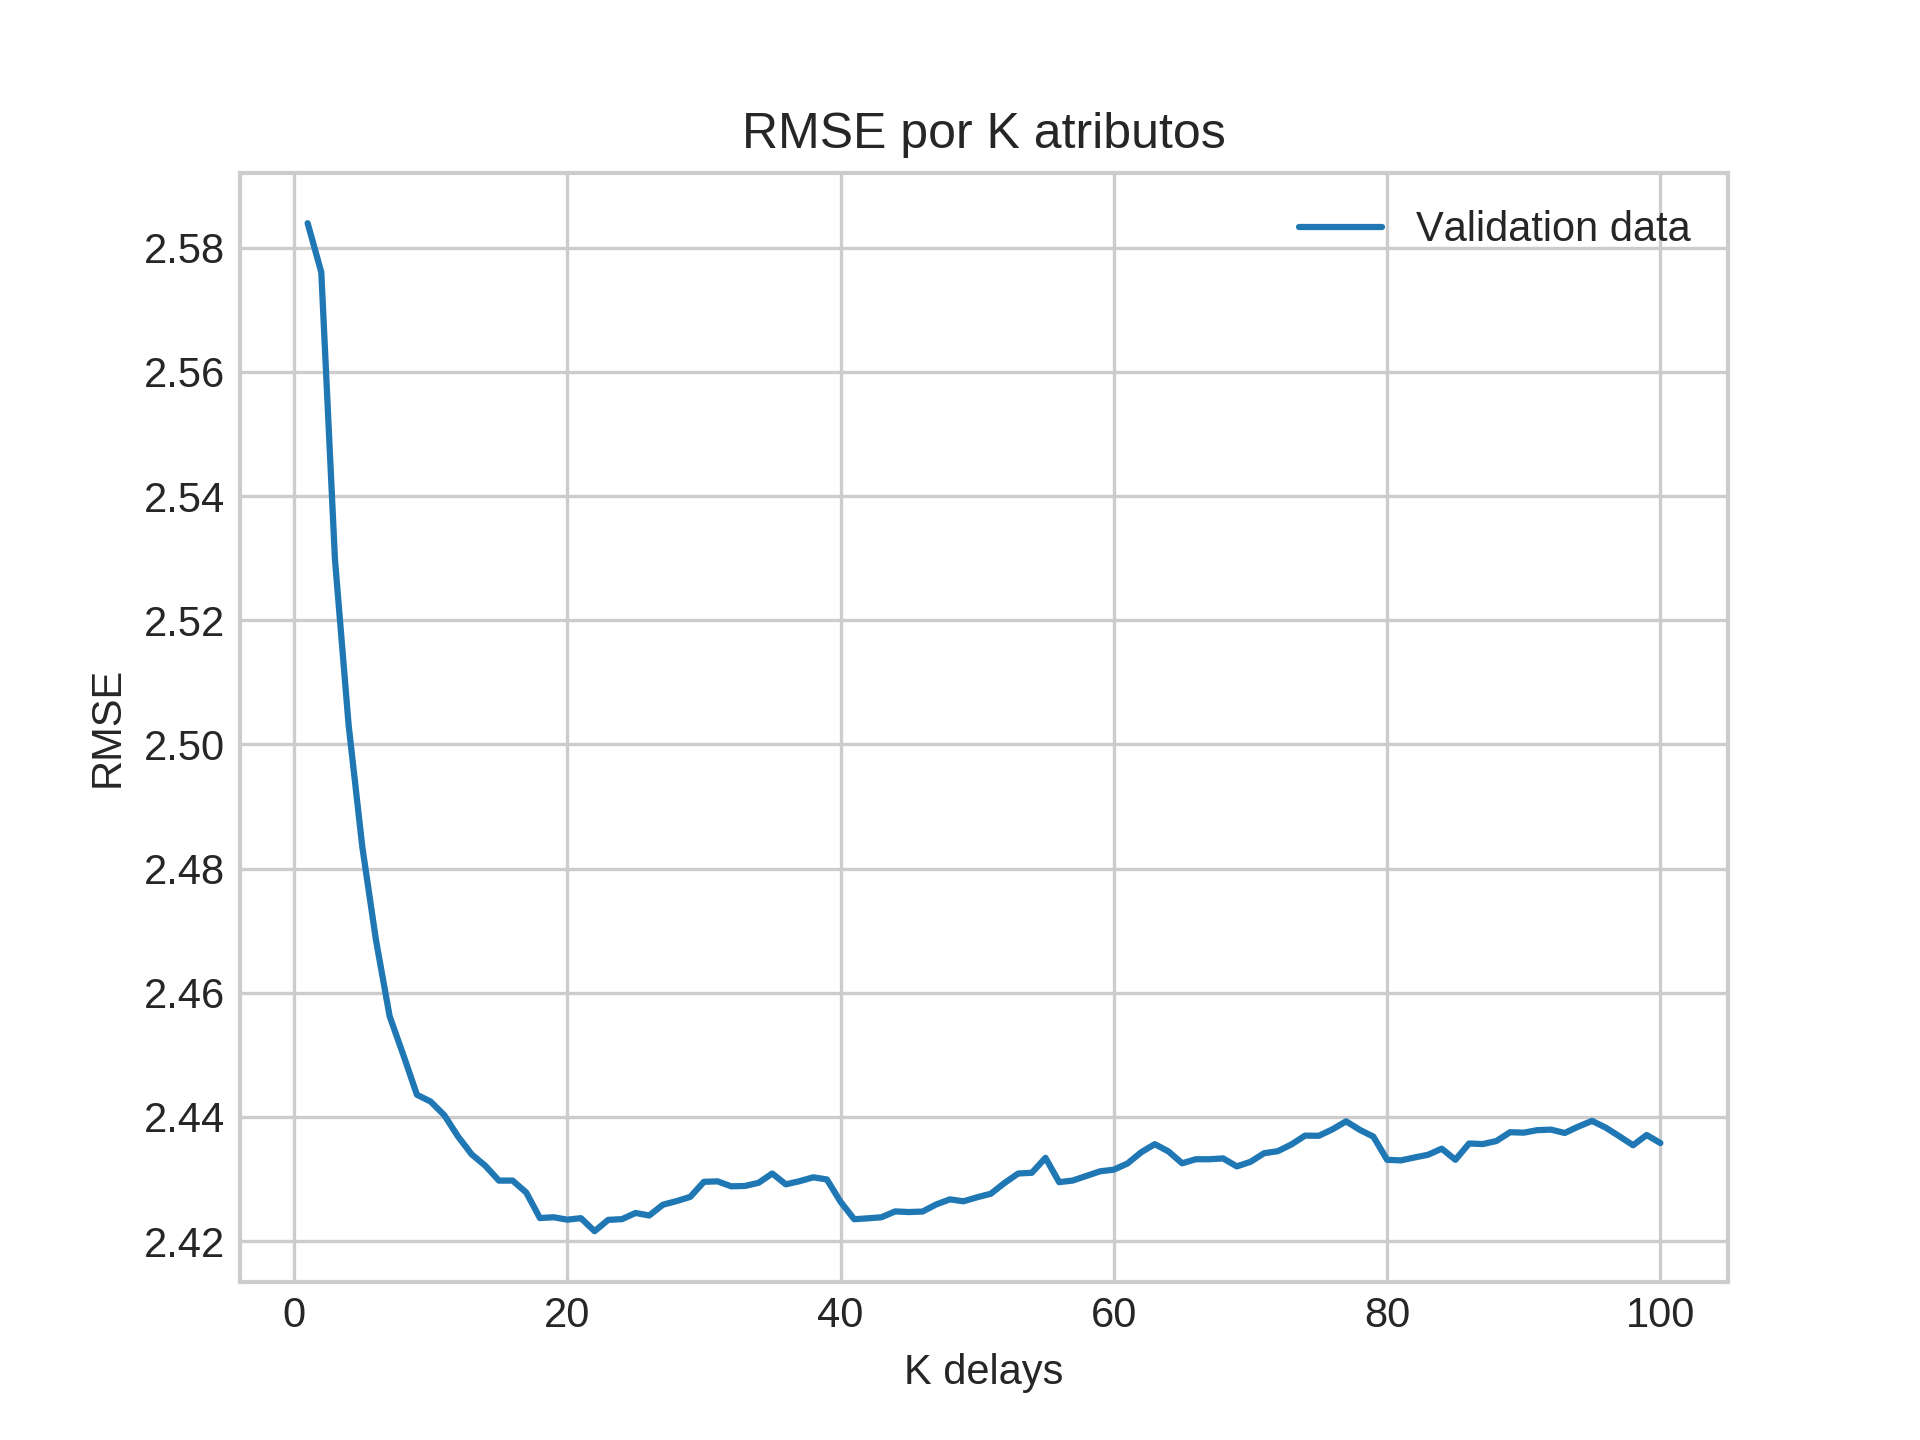
\includegraphics[width=\linewidth]{ex01/folds.png}
        \caption{Exercício 01: RMSE com validação cruzada \textit{10-folds} para $K$ \textit{delays}.}
        \label{fig:ex1_kfold_rmse}
    \end{figure}
    O número de atrasos $K$ que apesentou menor erro quadrático médio durante a validação dos modelos foi:
    \begin{align}
        K&=22\\
        RMSE&=2.4215989698821407
    \end{align}
    Definido o número de atributos $K$ um novo modelo é calculado
    utilizando todos os dados que não foram reservados para testes.
    \begin{align*}
w=[ &0.60851412, 0.58768129, -0.08816496, 0.05312793, 0.03412434, 0.04066411, \\
    &0.028874  , 0.04560297,  0.01880947, 0.0336419,  0.00261787, 0.00780726, \\
    &0.01769519, 0.02374471,  0.00350507,  0.02043056,0.01260365, 0.0110618,  \\
    & 0.04655714, -0.00340386,  0.02787026,  0.01283307,  0.00674837]^T
    \end{align*}
    Uma vez obtido o vetor de pesos $w$ do preditor, o \textit{dataset} de testes é utilizado para
    sua avaliação final. É possivel observar \ref{fig:ex1_model_comp} que o preditor, apesar dos erros de estimação, modelou a dinâmica dos dados.
    
    Do teste realizado, foram obtidos erros de estimação \ref{fig:ex1_kfold_rmse} com as seguintes características:
   \begin{align}
       \sigma^2&=2.0928243101998594\\
       \sigma&=1.7478639423536222\\
       \mu&=1.4466597078096353\\
       min(RMSE)&=0.0015856919462313712\\
       max(RMSE)&=7.12356630491203 
   \end{align}

   \begin{figure}[!h]
        \centering
        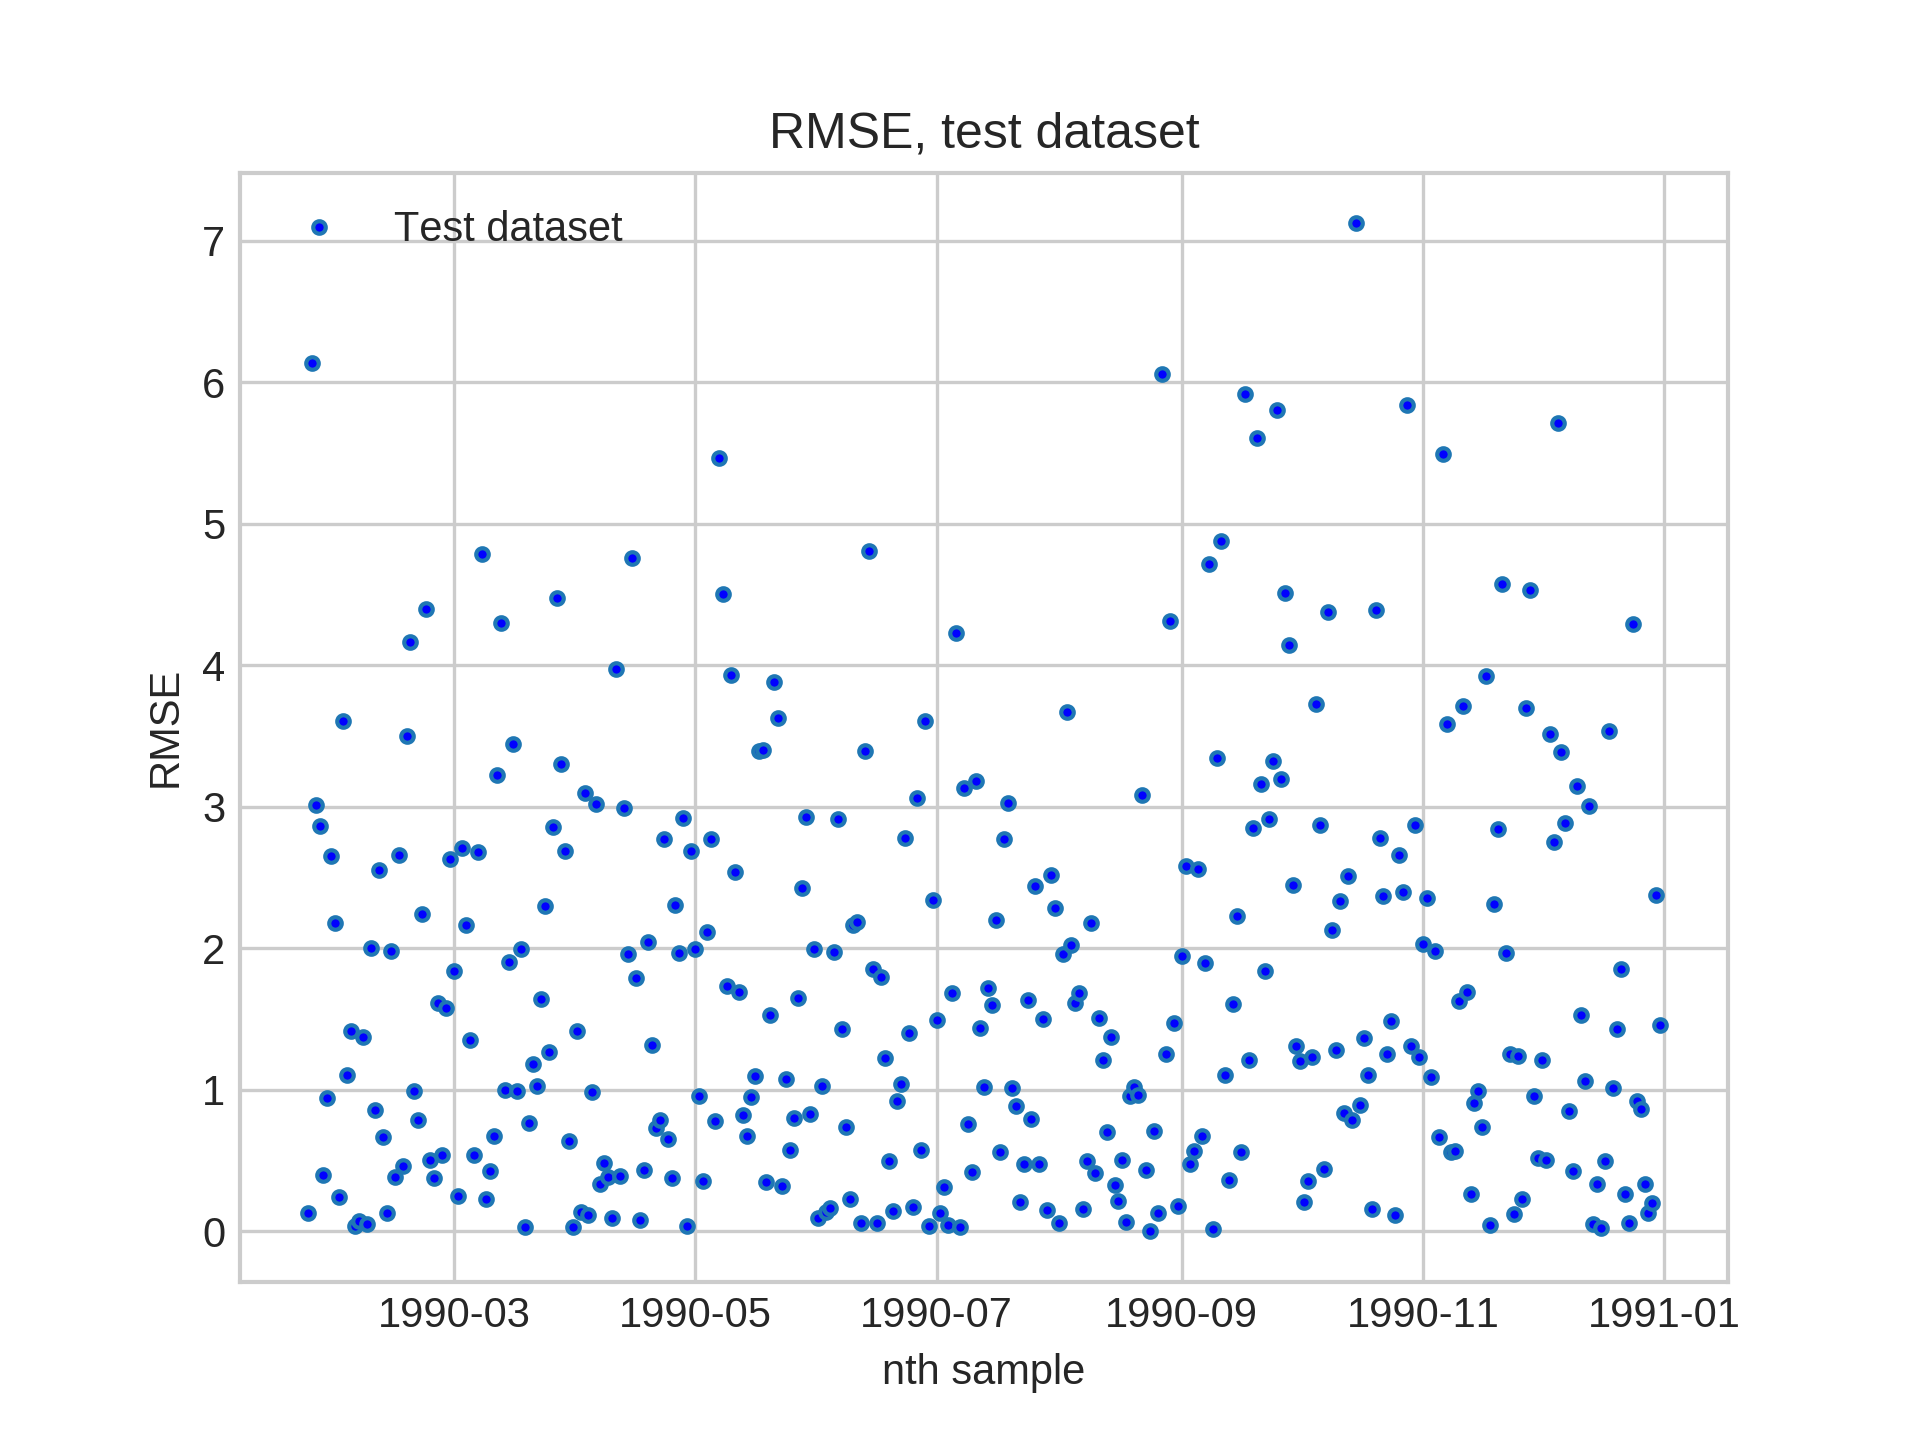
\includegraphics[width=\linewidth]{ex01/model.png}
        \caption{Exercício 01: RMSE do \textit{dataset} de teste para o modelo escolhido.}
        \label{fig:ex1_kfold_rmse}
    \end{figure}
    \begin{figure}[!h]
        \centering
        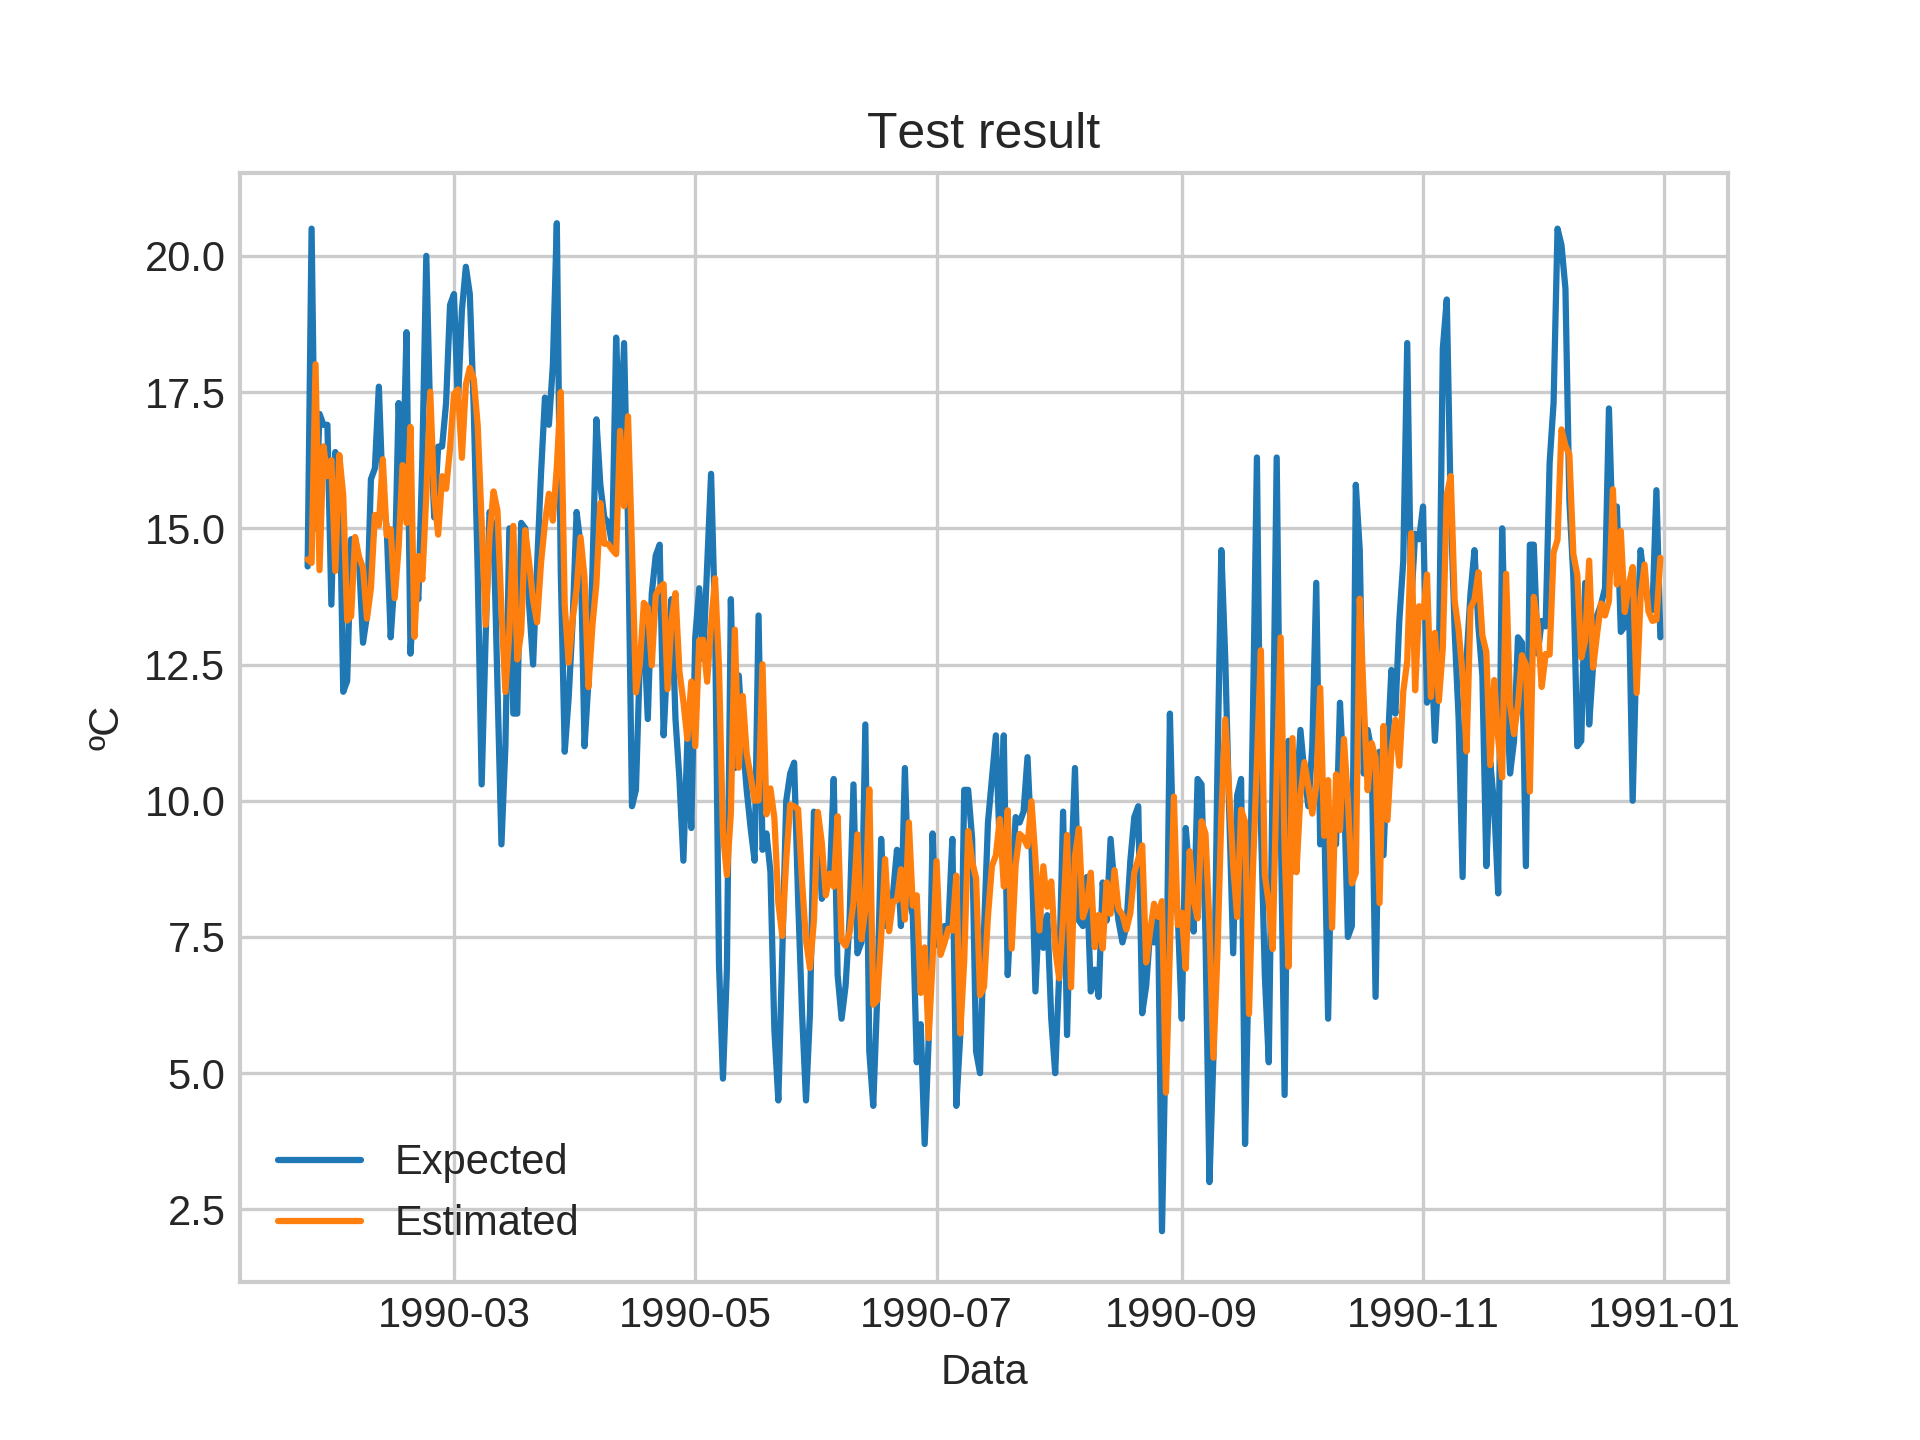
\includegraphics[width=\linewidth]{ex01/model_comp.png}
        \caption{Exercício 01: Estimação do modelo para o \textit{dataset} de teste e o valor esperado.}
        \label{fig:ex1_model_comp}
    \end{figure}


    \newpage
    \subsection[]{Exercício 02}
    \begin{figure}[!h]
        \centering
        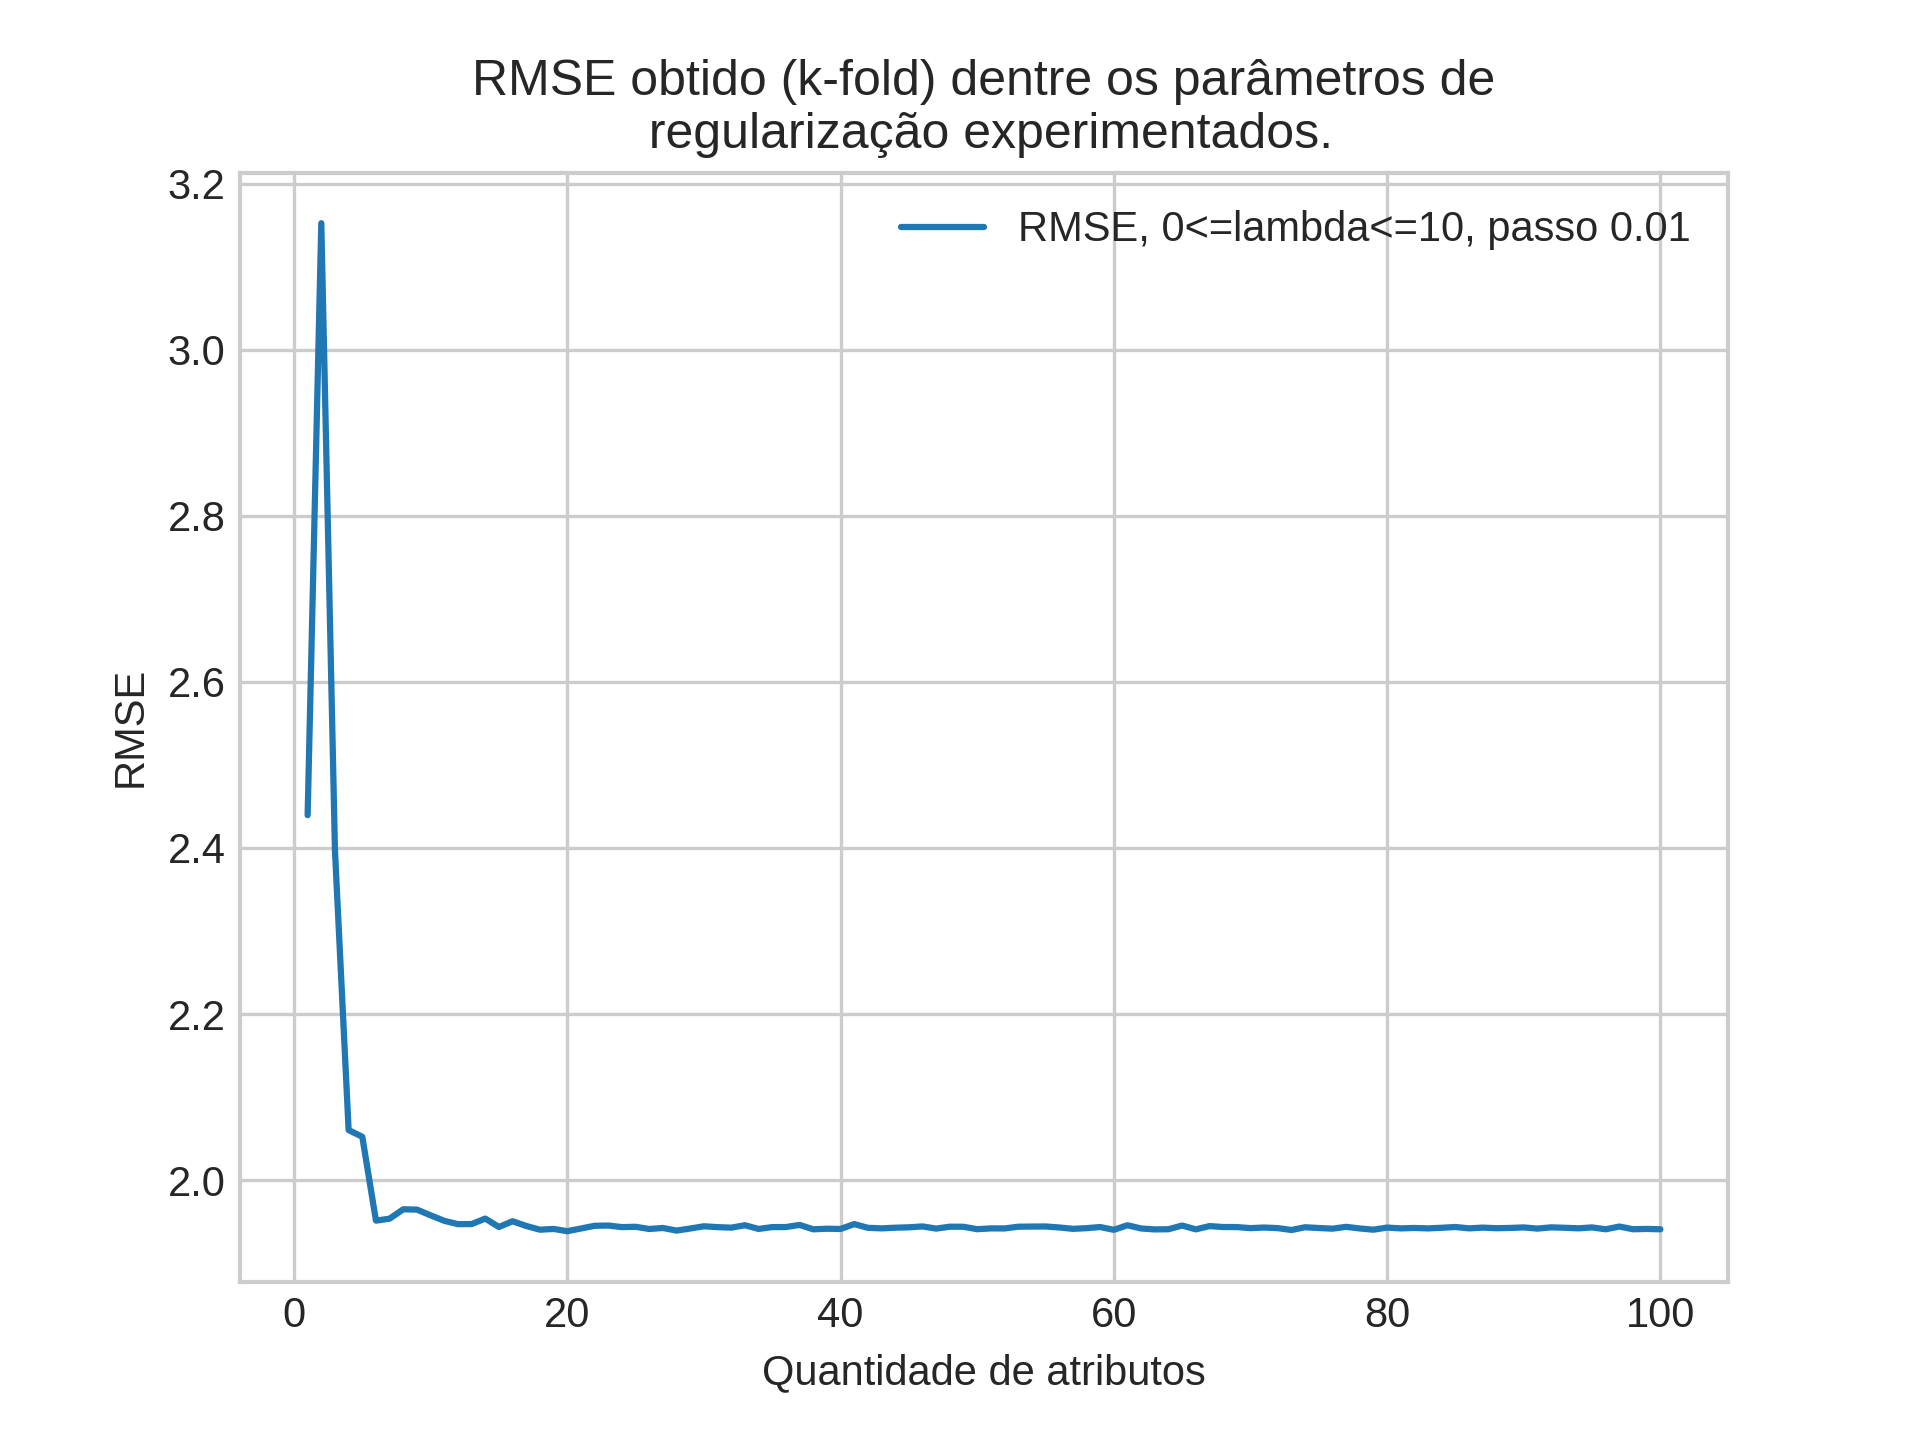
\includegraphics[width=\linewidth]{ex02/TsMeans.png}
        \caption{Exercício 02: RMSE em função do número de atributos $T$.}
        \label{fig:ex2_TRMSE}
    \end{figure}
    \begin{figure}[!h]
        \centering
        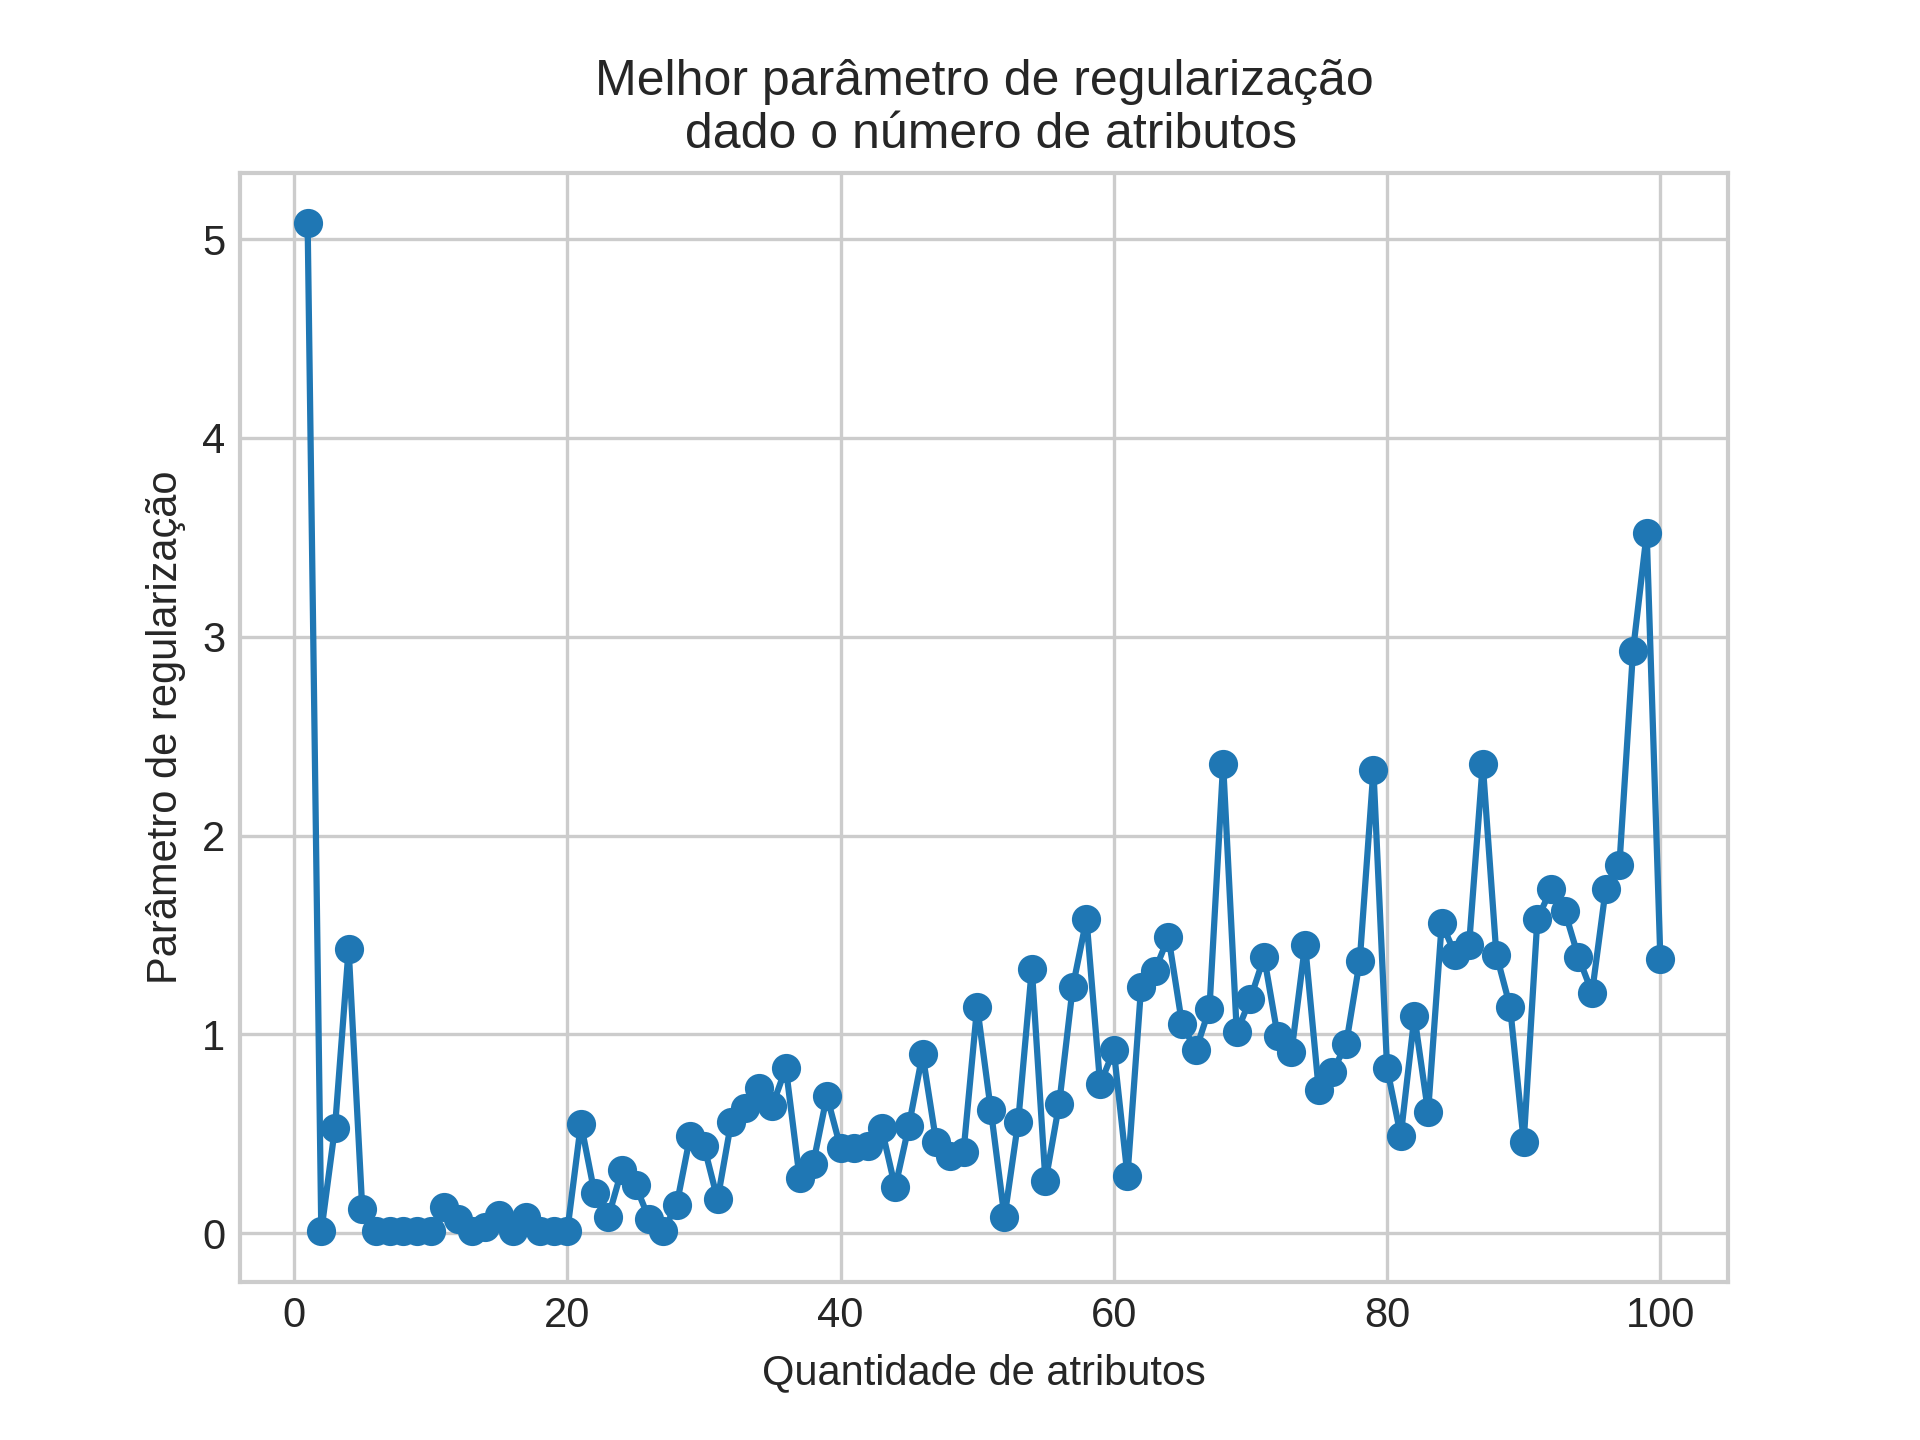
\includegraphics[width=\linewidth]{ex02/Tslambs.png}
        \caption{Exercício 02: Melhor $\lambda$ para dados $t$ atributos, sendo $t \leqslant T \leqslant $.}
        \label{fig:ex2_Tlamb}
    \end{figure}
    \begin{figure}[!h]
        \centering
        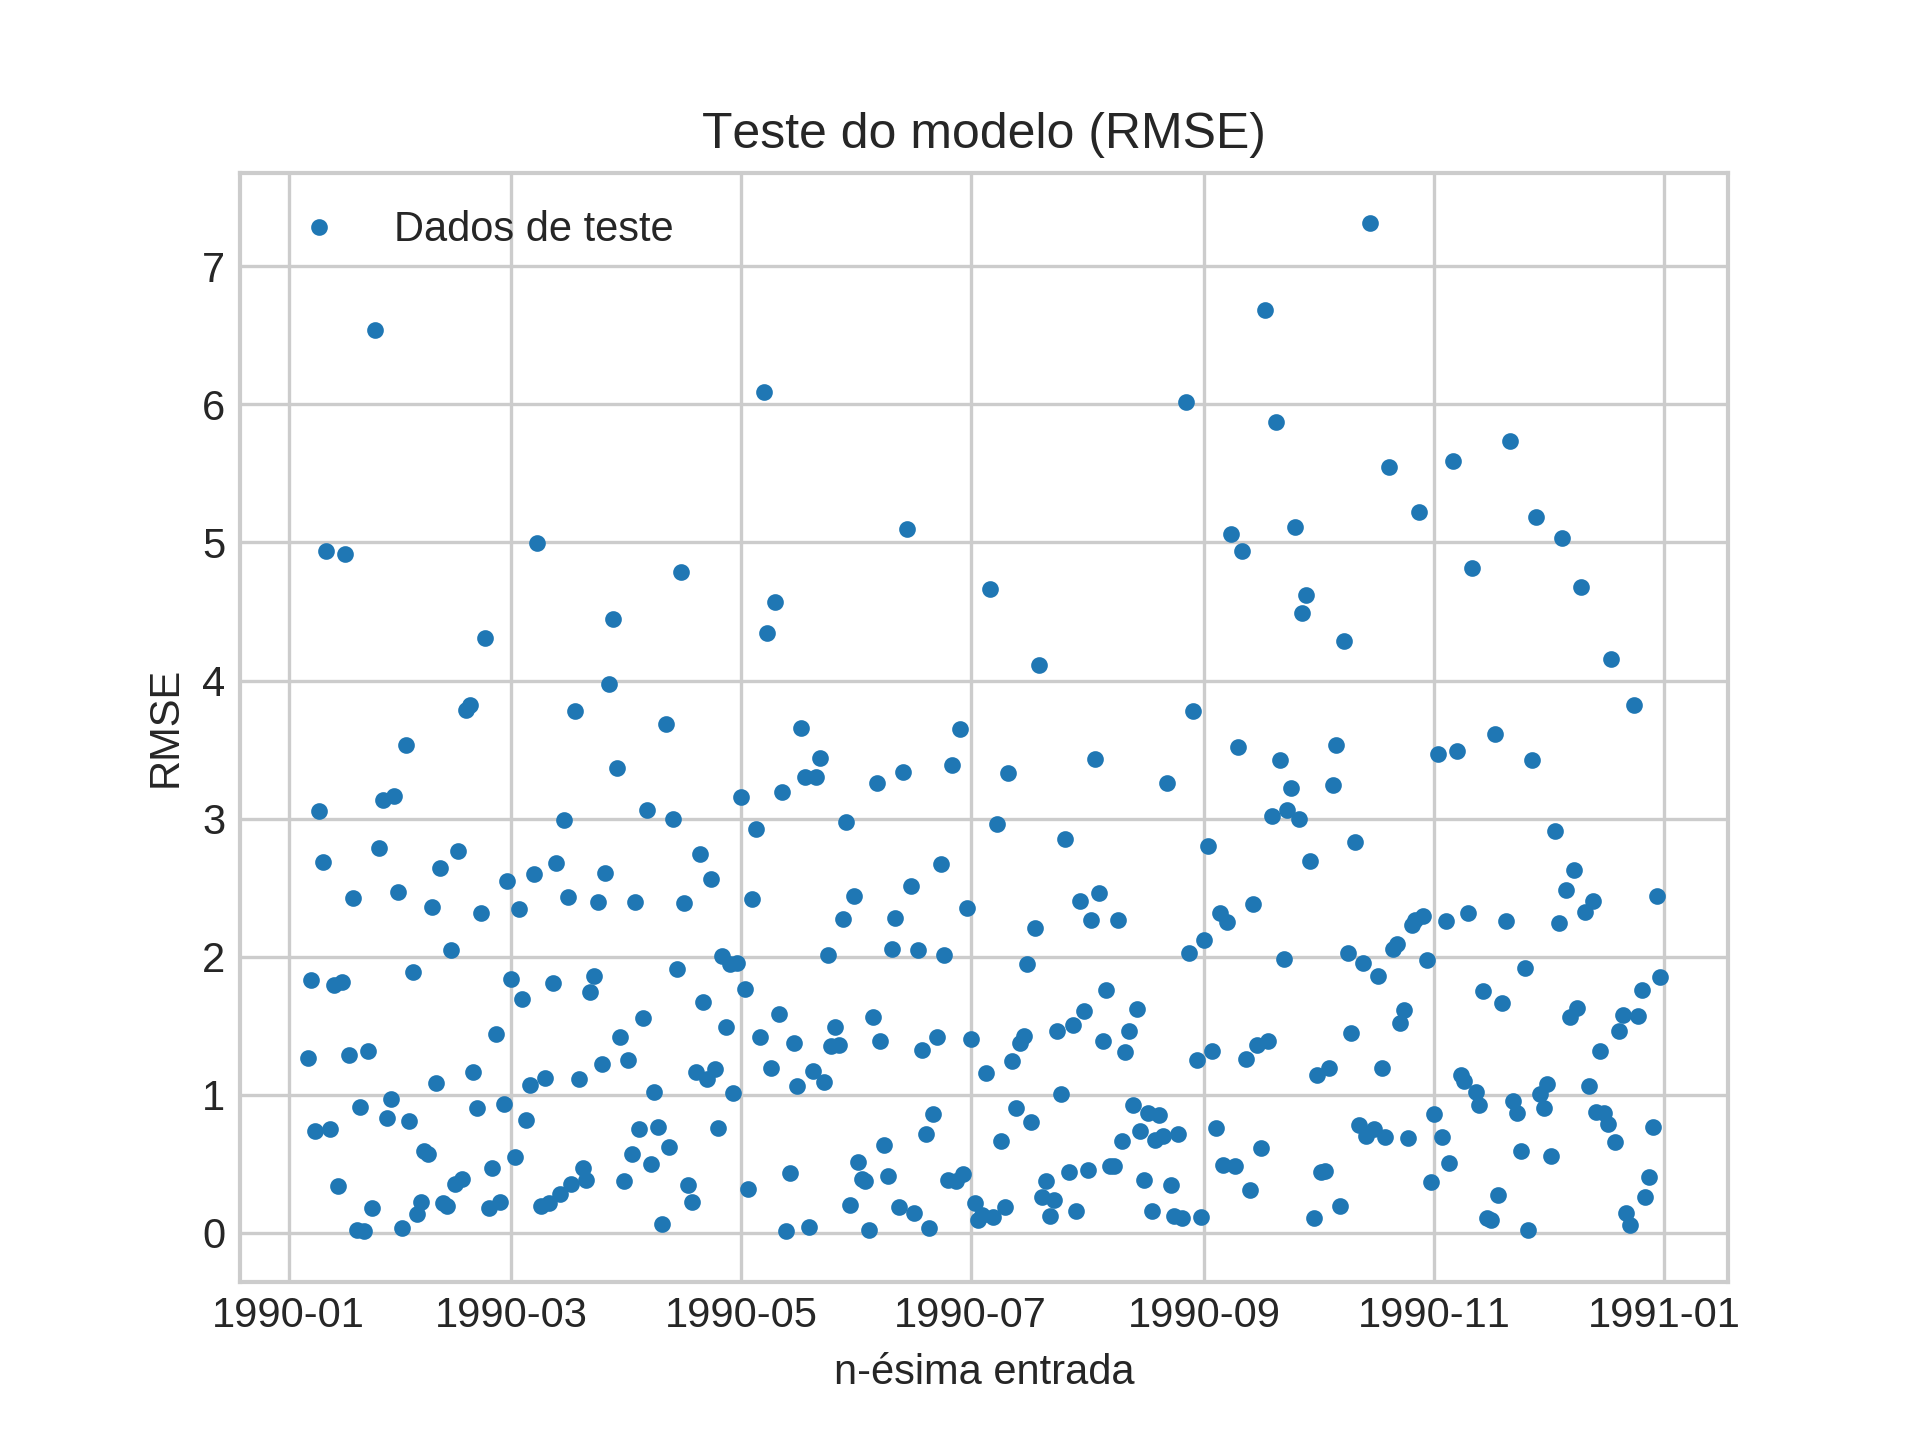
\includegraphics[width=\linewidth]{ex02/model_rmse.png}
        \caption{Exercício 02: RMSE do \textit{dataset} de teste para o modelo escolhido.}
        \label{fig:ex2_rmse}
    \end{figure}
    \begin{figure}[!h]
        \centering
        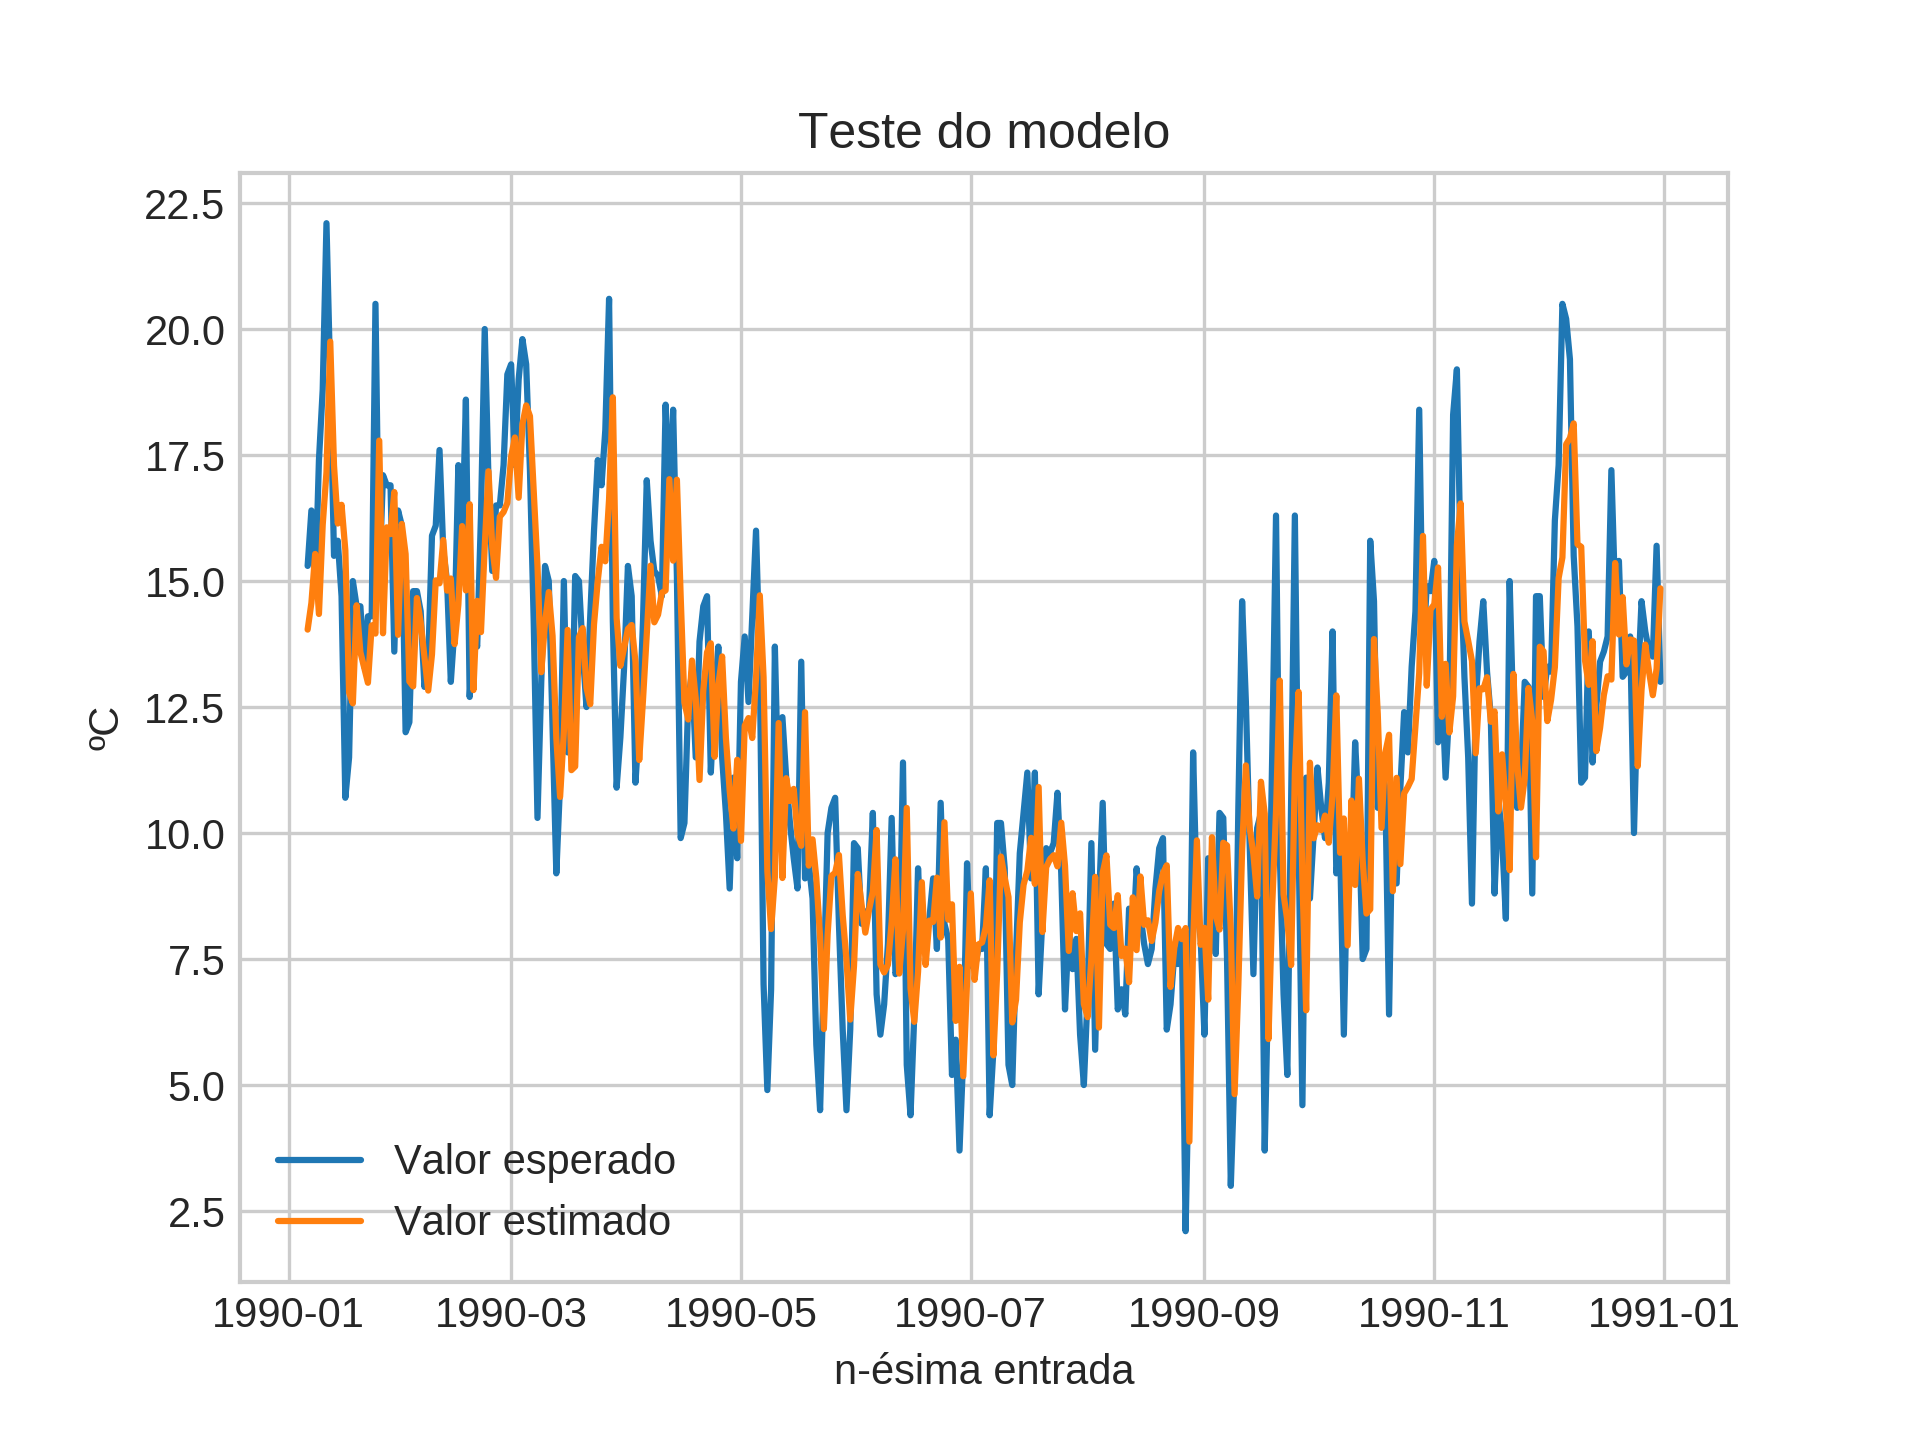
\includegraphics[width=\linewidth]{ex02/model_test.png}
        \caption{Exercício 02: Estimação do modelo para o \textit{dataset} de teste e o valor esperado.}
        \label{fig:ex2_comp}
    \end{figure}
\end{document}